\documentclass[12pt]{article}
\usepackage{graphicx}
\usepackage{hyperref}
\usepackage{cite}

\begin{document}
\title{CSE441 Semester Project: FunCoin}
\author{Rob Kelly\\Sean Turner\\Randy Van Why}
\maketitle

\section{Background}
In October of 2008, a white paper\cite{nakamoto:bitcoin} describing Bitcoin, a decentralized peer-to-peer electronic cash system, was published through cryptography mailing lists.

\section{OpenSSL}
The group used OpenSSL to handle most of the cryptographic functionality. OpenSSL provides a nice interface for performing digital signitures using DSA.

\section{Approach}\label{approach}
The basic approach we took was to familiarize ourselves with the Bitcoin paper\cite{nakamoto:bitcoin} and the Bitcoin Developer Guide \cite{dev:guide}. 

\subsection{Block Chain}\label{blockchain}
Figure \ref{figblockchain} (from the developer guide) sums up the basic structure of the blockchain nicely. 

\begin{figure}[h!]\label{figblockchain}
	\centering
	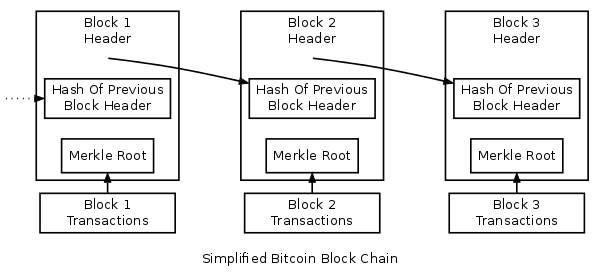
\includegraphics[scale=0.5]{en-blockchain-overview.png}
	\caption{Simplified block chain overview from \cite{dev:guide}}
\end{figure}

The blockchain constitutes the public ledger. It keeps transactions in order with timestamps and provides protection against double spending. The heart of the blockchain is the Merkle tree. As can be seen in Figure \ref{figblockchain}, every block holds the root of this Merkle tree. This significantly improves the storage complexity of the blockchain since the Merkle root is a small and easily transmitted piece of data that describes all the transactions in the block. And since the block header already contains the hash of the previous block header, this gives us all the information we need about transactions. 


Our blockchain consists of a simplified Merkle tree-like tree structure that doesn't do anything fancy cryptographically speaking. Our ``transactions" are just human readable strings detailing where fundoshis went and how many. This way, the ``merkle root" can just be actually read, and the whole structure of the block chain is simple to understand.

\section{Discussion}\label{future}
\subsection{Future Work}\label{work}
Some work that can be done to our implementation includes extending it from a simple client/server model to a true peer-to-peer cryptocurrency, making it more modular, so that interested parties may substitute their own implementations of key components such as the block chain and the proof of work in order to gain better understanding of the underlying techniques, and implement true transactions. 

Additional future projects include: implementing a wallet, considering different mining techniques altogether, and following on modularity, possibly making it into a library that can be used to roll your own simplified fun coin.

\subsection{Unsolved Problems}\label{unsolved}
Our biggest unsolved problem (and opportunity for Section \ref{future}) is to decentralize for a more accurate portrayal of how real cryptocurrencies function. Additionally, 

\bibliographystyle{abbrv}
\bibliography{report}

\end{document}
